%==========================================================
% Preamble
%==========================================================
% Fonts/languages
\documentclass[english,aspectratio=169,12pt,xcolor=dvipsnames]{beamer}
%\usepackage[orientation=landscape,size=custom,width=16,height=9,scale=0.45,debug]{beamerposter} % change to 16x9 aspect ratio from default 4x3
\usepackage[T1]{fontenc}
\usepackage[latin9]{inputenc}
\usepackage{babel}            % For bibliographies

\usepackage[scaled]{beramono}  % Load typewriter font first, since Arial doesn't have one
\usepackage{helvet}            % For Arial font
\renewcommand{\familydefault}{\sfdefault}
%\renewcommand{\ttfamily}{beramono}

%\usepackage{mathpazo}         % For Palatino font
%%\usepackage{mathptmx}         % For Times New Roman font
%\usefonttheme{serif}          % To have a serif font (instead of Beamer's default sans serif)

% Colors: see  http://www.math.umbc.edu/~rouben/beamer/quickstart-Z-H-25.html
\usepackage{color}
\usepackage[dvipsnames]{xcolor}
\definecolor{dgreen}{rgb}{0.,0.6,0.}
\definecolor{forest}{RGB}{34.,139.,34.}
\definecolor{byublue}{RGB}{0.,30.,76.}
\definecolor{dukeblue}{RGB}{0.,0.,156.}
\definecolor{oucrimson}{RGB}{132.,22.,23.}

% Beamer Themes
%\usetheme{Ilmenau}
%%%%%%%%%%%%%%%%%%%%%%%%%%%%%%%%%%%%%%%%%%%%%%%%
% NOTE: With Ilmenau style, to get the bullets %
% looking right, do one section and one sub-   %
% section for each set of bullets              %
% This is not necessary with Frankfurt         %
%%%%%%%%%%%%%%%%%%%%%%%%%%%%%%%%%%%%%%%%%%%%%%%%

\usetheme{CapeTown}
\setbeamercolor{section in head/foot}{bg=oucrimson,fg=white}  % use this to adjust the coloring of CapeTown
\setbeamercolor{frametitle}{bg=white,fg=oucrimson}            % use this to adjust the coloring of CapeTown
\setbeamercolor{alerted text}{fg=oucrimson}
\usecolortheme[named=oucrimson]{structure}                   % change the color theme
%\usecolortheme[named=RawSienna]{structure}                  % change the color theme
%\usecolortheme[named=byublue]{structure}                    % change the color theme
%\setbeamertemplate{itemize items}[default]                  % change bullet style. options are: default (triangle), square, circle, ball
\setbeamercovered{invisible}

%\usetheme{Frankfurt}
%\setbeamercolor{section in head/foot}{fg=white,bg=byublue}  % use this to adjust the coloring of Frankfurt
%\usecolortheme[named=dukeblue]{structure}                   % change the color theme
%%\usecolortheme[named=RawSienna]{structure}                 % change the color theme
%%\usecolortheme[named=byublue]{structure}                   % change the color theme
%\setbeamertemplate{navigation symbols}{}                    % remove annoying navigation symbols
%%\setbeamertemplate{headline}{}                             % remove header line
%\setbeamertemplate{footline}{}                              % remove footer line
%\setbeamercovered{invisible}                                % transparent shows bullets in gray; invisible hides bullets
%
%\usepackage{remreset}                                       % For FRANKFURT (and ILMENAU) style
%\makeatletter                                               % to allow circles
%\@removefromreset{subsection}{section}                      % to appear by frame
%\makeatother                                                % instead of by
%\setcounter{subsection}{1}                                  % subsection.

% Layout
%\usepackage[bottom]{footmisc}                         % Forces footnotes on bottom

% Useful Packages
%\usepackage{bookmark}                                              % For speedier bookmarks
\usepackage{booktabs}                                              % For more professional tables
\usepackage{babel}                                                 % For multilingual output
\usepackage{amsthm}                                                % For detailed theorems
\usepackage{amssymb}                                               % For fancy math symbols
\usepackage{amsmath}                                               % For awesome equations/equation arrays
\usepackage{float}                                                 % For improved float manipulation
\usepackage{prettyref}                                             % For pretty references
\usepackage{array}                                                 % For tubular tables
\usepackage{longtable}                                             % For long tables
\usepackage[flushleft]{threeparttable}                             % For three-part tables
\usepackage{multicol}                                              % For multi-column cells
\usepackage{graphicx}                                              % For shiny pictures
\usepackage{subfig}                                                % For sub-shiny pictures
\usepackage{enumerate}                                             % For cusomtizable lists
\usepackage{listings}                                              % For ``verbatim'' code
%\usepackage{outline}                                               % For an outline environment (similar to enumerate, but can go six levels deep)
\usepackage{pdflscape}                                             % For landscape-oriented pages
%\usepackage{pstricks,pst-node,pst-tree,moredefs}                   % For trees
%\usepackage{tikz,pgfplots}                                         % For tikz figures
%\pgfplotsset{compat=1.7}
%\pgfplotsset{scaled y ticks=base 10:2}

% Custom operators for variance, covariance, and correlation
\newcommand{\Var}{\operatorname{Var}}
\newcommand{\Cov}{\operatorname{Cov}}
\newcommand{\Corr}{\operatorname{Corr}}

% Bib
\usepackage[authoryear]{natbib}                                    % Bibliography
\renewcommand{\bibsection}{\subsubsection*{\bibname } }            % Allows Bibliographies in Beamer
\usepackage{url}                                                   % Allows urls in bib

% Links
\usepackage{hyperref}                                              % Always add hyperref (almost) last
%\hypersetup{unicode=true,bookmarksnumbered=true,bookmarksopen=true,bookmarksopenlevel=4,
% breaklinks=true,pdfborder={0 0 0},colorlinks=false,citecolor=black,filecolor=black,linkcolor=black,urlcolor=black}
\hypersetup{unicode=true,breaklinks=true,pdfborder={0 0 0}}

% Julia definition (c) 2014 Jubobs
%\lstdefinelanguage{Julia}%
%  {morekeywords={abstract,begin,break,case,catch,const,continue,do,else,elseif,%
%      end,export,false,for,function,immutable,import,importall,if,in,%
%      macro,module,otherwise,quote,return,switch,true,try,type,typealias,%
%      using,while},%
%   sensitive=true,%
%   alsoother={$},%
%   morecomment=[l]\#,%
%   morecomment=[n]{\#=}{=\#},%
%   morestring=[s]{"}{"},%
%   morestring=[m]{'}{'},%
%}[keywords,comments,strings]%

%\lstset{%
%    language         = Julia,
%    basicstyle       = \ttfamily,
%    keywordstyle     = \bfseries\color{blue},
%    stringstyle      = \color{magenta},
%    commentstyle     = \color{ForestGreen},
%    showstringspaces = false,
%}

%%==========================================================
%%Change bullet spacing Chetty-style:
%\makeatletter
%\newcommand{\setlistspacing}[2]{\def\@ld{#1}\expandafter\def\csname
%@list\romannumeral\@ld \endcsname{\leftmargin\csname
%leftmargin\romannumeral\@ld \endcsname
              %\topsep    #2
              %\parsep    0\p@   \@plus\p@
              %\itemsep   #2}}
%\makeatother
%\setlistspacing{1}{2.5ex}
%%==========================================================

%==========================================================
% How to cite an author using BibTeX:
% \citet{hotz_et_al2002} --> Hotz et al. (2002)
% \citeauthor{hotz_et_al2002} ---> Hotz et al.
% \citep{hotz_et_al2002} --> (Hotz et al., 2002)
% \citealp{hotz_et_al2002} --> Hotz et al., 2002
% \citealt{hotz_et_al2002} --> Hotz et al. 2002
% \citeyear{hotz_et_al2002} --> 2002
% \citeyearpar{hotz_et_al2002} --> (2002)
% \nocite{hotz_et_al2002} --> [only shows up in bibliography]
%
% If you add a "*" to the command, it will list all authors:
% \citet*{hotz_et_al2002} --> Hotz, Xu, Tienda, and Ahituv (2002)
% \citeauthor*{hotz_et_al2002} ---> Hotz, Xu, Tienda, and Ahituv
% \vdots
% etc.
%==========================================================

%==========================================================
% How to use overlay specifications in Beamer:
%
% Overlay specifications are given in pointed brackets (<,>) and
% indicate which slide the corresponding information should appear
% on.
% The specification <1-> means ``display from slide 1 on.'' <1-3>
% means ``display from slide 1 to slide 3.'' <-3,5-6,8-> means
% ``display on all slides except slides 4 and 7.''
% Here is an example:
% \begin{itemize}
% \item<1> $abcadcabca$
% \item<1-2> $abcabcabca$
% \item<1-2> $accaccacca$
% \item<1> $bacabacaba$
% \item<1,3> $cacdaccacc$
% \item<1-2> $caccaccacc$
% \end{itemize}
%==========================================================

%==========================================================
% How to add ToC before each section:
\AtBeginSection[]{
 \frame<beamer>{ 
   \frametitle{Outline}   
   \tableofcontents[currentsection] 
}
}
%==========================================================

\title{What is Data Science?}
\author{Tyler Ransom}
\institute[OU Econ]{\normalsize{University of Oklahoma, Dept. of Economics}}
\date{January 14, 2020}

\begin{document}

{
\setbeamertemplate{footline}{} 
\frame[noframenumbering]{\titlepage}
}

\AtBeginSection[] {
\begin{frame}
    \frametitle{Outline}
    \tableofcontents[currentsection]
\end{frame}
}

\section{Intro}
\begin{frame}{What is data science?}
\begin{itemize}
\item \alert{Data science (DS):} The scientific discipline that deals with transforming data into useful information (``insights'') using a variety of statistical and machine learning techniques
    \begin{itemize}
    \item \alert{Amazon:} Collects data on search history, cart history, purchases
    \item Analyzes the data to estimate users' willingness to pay for various products (including Prime); recommend new products
    \end{itemize}
\item The rise of data science has come because of the so-called Big Data revolution
    \begin{itemize}
    \item The rise of the internet in the late-1990s and 2000s $\Rightarrow \,\uparrow$opportunities for companies and governments to collect data on consumers \& citizens
    \item Proliferation of mobile devices \& social media from late 2000s until now has generated even more data
    \end{itemize}
\end{itemize}
\end{frame}


\begin{frame}{Skills required for data science}
\begin{center}
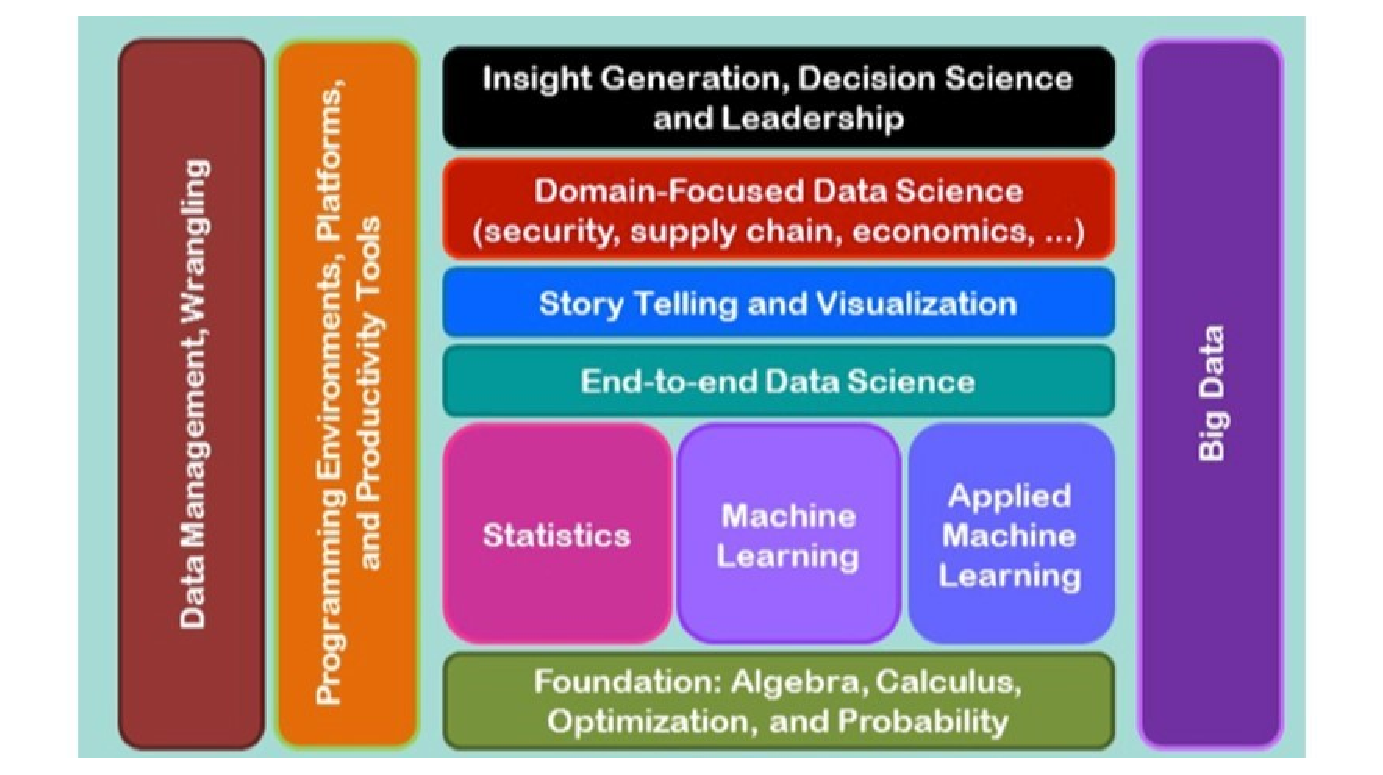
\includegraphics[width=0.76\textwidth]{../Graphics/NASEMdatasci.eps}
\end{center}
{\scriptsize Source: \href{http://sites.nationalacademies.org/cs/groups/cstbsite/documents/webpage/cstb_181680.pdf}{NC State Univ.} (p. 26)}
\end{frame}

\begin{frame}{Pillars of data science}
\begin{itemize}
\item Programming (for automation of data collection, manipulation, cleaning, visualization, and modeling)
\item Visualization \& exploration
\item Machine learning (to select models, compress data)
\item Causal inference (to be able to make a policy prescription)
\end{itemize}
...Assuming one has the appropriate foundation of basic calculus and statistics
\end{frame}


\begin{frame}{The data science workflow}
\begin{center}
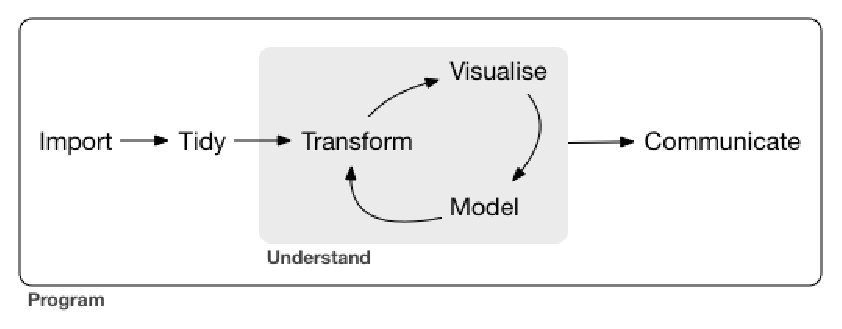
\includegraphics[width=0.85\textwidth]{../Graphics/data-science.eps}
\end{center}
{\scriptsize Source: \href{{http://r4ds.had.co.nz/introduction.html}}{\emph{R for Data Science}}}
\end{frame}

\section{Big Data}
\begin{frame}{What is Big Data?}
\visible<1->{
\begin{center}
\includegraphics<1->[width=0.85\textwidth]{../Graphics/frisch.eps}
\end{center}
}
\visible<2->{
{\scriptsize Source: Frisch, Ragnar. 1933. ``Editor's Note'' \emph{Econometrica} 1(1): 1--4}
}
\end{frame}


\begin{frame}{What is Big Data?}
It depends on who you ask. It could mean:
\begin{enumerate}
\item ``Wild'' data (unstructured; collected without a particular intention; e.g. twitter, contrast with Census surveys)
\item ``Wide'' data (a.k.a. ``Big-K'' data because $K>N$)
\item ``Long'' data (a.k.a. ``Big-N'' data because $N$ very, very large [and may not all fit onto a single hard drive!])
\item Any data set that cannot be analyzed with classical methods like OLS (e.g. all combinations of the above three types)
\end{enumerate}
``Big Data'' not so much about size of data (after all, Moore's Law is giving us higher-capacity hard drives every year!), but about whether or not ``small data'' (read: classical) methods can be used
\end{frame}

\section{Machine Learning}
\begin{frame}{What is machine learning? What is AI?}
\begin{itemize}
\item \alert{Machine learning (ML):} Allowing computers to learn for themselves without explicitly being programmed
    \begin{itemize}
    \item \alert{USPS:} Computer to read handwriting on envelopes
    \item \alert{Google:} AlphaGo, computer that defeated world champion Go player
    \item \alert{Apple/Amazon/Microsoft:} Siri, Alexa, Cortana voice assistants 
    \end{itemize}
\item \alert{Artificial intelligence (AI):} Constructing machines (robots, computers) to think and act like human beings
\item ML is a subset of AI
\end{itemize}
\end{frame}


\begin{frame}{Big data \& machine learning}
\begin{itemize}
\item You'll often hear the phrase ``big data and machine learning''
\item This is because many machine learning algorithms are helpful for big data problems:
    \begin{itemize}
    \item Selecting which $k<K$ covariates should enter your model
    \item Streamlined techniques for processing ``wild'' data
    \item New modeling approaches that can leverage the greater amount of information that Big Data has
    \end{itemize}
\end{itemize}
\end{frame}

\section{Causality}
\begin{frame}{Correlation vs. causation}
\begin{itemize}
\item Machine learning is not the end-all, be-all of data science
\item A good data scientist knows that correlation is not causation!
\item Ultimately companies want ``insights'' that they can use to $\uparrow$profits
\item Tech co.'s run randomized experiments to estimate causal effects
\item Can also estimate fancier statistical models to account for selection
\item Economists' comparative advantage is in combining machine learning with economic theory to produce optimal policies
\end{itemize}
\end{frame}

\begin{frame}{Example}
\begin{quote}
One very classic example comes from looking at the data of a shopping cart. Why do sales of beer and diapers go hand in hand? The correlation is women tell their husbands to go pick up diapers, and on the way, they pick up beer, too. That is data science: finding trends from your data and using that insight to increase your sales or market better
\end{quote}
Source: \url{http://www.chicagotribune.com/bluesky/originals/ct-bsi-inside-job-4c-insights-20171002-story,amp.html}
\end{frame}

\section{Jobs}
\begin{frame}{Lifestyle}
\begin{itemize}
\item What's it like to have a DS job right now: \url{http://www.businessinsider.com/what-its-like-to-be-a-data-scientist-best-job-in-america-2017-9/\#why-data-scientists-have-the-best-job-1}
\item Research from 1,001 data scientist job profiles: \url{https://www.kdnuggets.com/2017/12/research-1001-data-scientist-profiles.html}
\end{itemize}
\end{frame}

\section{Project}
\begin{frame}{Final project}
\begin{itemize}
\item A large portion of your grade will come from a final project
\item You should find a research question you're interested in and some data you can use to answer it
\item If you are short on ideas, check out \url{https://www.kaggle.com/datasets} which routinely hosts analytics competitions
\item Kaggle publishes data for each competition
\item Main criterion for the project is to apply skills developed in this class
\item If you have more questions, please come see me
\end{itemize}
\end{frame}

\appendix

\section*{Bonus slides}

%\begin{frame}[noframenumbering]{References}
%\bibliographystyle{jpe}
%\bibliography{biblio}
%\end{frame}

\end{document}
